\documentclass[a4paper,10pt,twocolumn]{article}

\usepackage[utf8x]{inputenc}
\usepackage[french]{babel}
\usepackage{graphicx,times}
\usepackage[T1]{fontenc}
\usepackage{amsmath}
\usepackage[font=footnotesize]{caption}
\usepackage{fancyhdr}
\usepackage[explicit]{titlesec}
\usepackage{hyperref}
%\usepackage[square,comma,numbers]{natbib}
\usepackage{tabularx}

% Petits extras:
\usepackage{textcomp} % Symbole Euro € \texteuro

\newcolumntype{L}[1]{>{\raggedright\arraybackslash}p{#1}}
\newcolumntype{C}[1]{>{\centering\arraybackslash}p{#1}}
\newcolumntype{R}[1]{>{\raggedleft\arraybackslash}p{#1}}

%\renewcommand{\bibsection}{}
%\def\bibfont{\footnotesize}
%\setlength{\bibsep}{0.2em}
%\setlength{\bibhang}{10em}

\hypersetup{colorlinks=true, urlcolor=blue, urlbordercolor={0 0 1}, citecolor=black, citebordercolor={1 1 1}}

\addto\captionsfrench{\def\figurename{Fig.}}
\addto\captionsfrench{\def\tablename{Tableau}}

\captionsetup[figure]{labelsep=period, justification=raggedright, singlelinecheck=false}
\captionsetup[table]{labelsep=period, justification=centering, singlelinecheck=false}

\parindent 10pt

\setlength{\voffset}{-1.3in}
\setlength{\topmargin}{1.25cm}
\setlength{\headheight}{1.125cm}
\setlength{\headsep}{0cm}

\setlength{\hoffset}{-1in}
\setlength{\oddsidemargin}{1.3cm}
\setlength{\evensidemargin}{1.3cm}

\setlength{\textheight}{25cm}%23.5
\setlength{\textwidth}{18.5cm}

\setlength{\headsep}{0.67cm}
\setlength{\columnwidth}{8.75cm}
\setlength{\columnsep}{0.63cm}

\setlength{\abovecaptionskip}{0em}
\setlength{\belowcaptionskip}{0em}

\titleformat{\section}
  {\normalfont}{\thesection.}{0.5em}{\MakeUppercase{#1}}
\titleformat{\subsection}
  {\normalfont\itshape}{\thesubsection.}{1.5em}{#1}
\titleformat{\subsubsection}
  {\normalfont\itshape}{\thesubsubsection.}{1.5em}{#1}
	
\titlespacing\section{0pt}{1em}{0.5em}
\titlespacing\subsection{0pt}{1em}{0.5em}
\titlespacing\subsubsection{0pt}{1em}{0.5em}

\fancyhf{}
\fancyhead[R]{\fontsize{8pt}{8pt}\selectfont \textbf{S}YMPOSIUM DE \textbf{G}ENIE \textbf{E}LECTRIQUE (SGE 2018), 3-5 JUILLET 2018, NANCY, FRANCE}
\renewcommand{\headrulewidth}{0pt}


\pagestyle{empty}


\title{
\fontsize{24pt}{24pt}\selectfont
Gestion d'énergie avec entrées incertaines : \\
quel algorithme choisir ?\\
Benchmark open source sur une maison solaire
}

\newcommand\tsp[1]{\textsuperscript{#1}}

\author{
\fontsize{11pt}{11pt}\selectfont
Pierre HAESSIG\tsp{*}, Jesse James PRINCE AGBODJAN\tsp{*}, Romain BOURDAIS\tsp{*}, Hervé GUÉGUEN\tsp{*}\\
\fontsize{10pt}{10pt}\selectfont
\tsp{*}IETR, CentraleSupélec
}

\date{}


\begin{document}

\maketitle
\thispagestyle{fancy}


\fontsize{9pt}{9pt}\selectfont
\textbf{RÉSUME --
Le pilotage optimal des systèmes énergétiques nécessite l'emploi d'algorithmes
de gestion optimale.
Ces outils se rattachent à théories de disciplines variées (Automatique, Optimisation, Recheche Opérationnelle),
qui ont chacune leur spécificité tout en se recouvrant partiellement.
%
Il est donc difficile, pour la personne ``non-initiée'', de saisir les principales caractéristiques
de chaque approche pour pouvoir les comparer et finalement trouver
quelles méthodes sont plus adaptées à un problème donné.
%
Pour permettre une comparaison objective et transparente,
nous proposons de problème simple de gestion d'énergie : une maison solaire 
avec production photovoltaïque et stockage, dont nous justifions le dimensionnement.
Ce benchmark accessible en ligne est open source et multi-langage (Python, Julia et Matlab).
Nous l'illustrons par une première comparaison de quelques méthodes de gestion d'énergie
(règle heuristique, MPC et optimisation anticipative)
et nous soulignons en particulier l'effet de l'incertitude
sur la production solaire.
% Extrait de l'ancien résumé, avec des idées à reprendre?
% comparer différentes méthodes en soulignant en particulier les investissements
% en temps à prévoir :
% temps pour la compréhension du cadre théorique,
% temps pour la modélisation du problème dans ce cadre,
% temps pour l'implémentation numérique et la validation des résultats.
}\\

\textbf{\textit{Gestion d'énergie, Optimisation dynamique, Optimisation stochastique,
Commande prédictive, Autoconsommation photovoltaïque}}

\fontsize{10pt}{10pt}\selectfont


\section{Introduction}

De très nombreux travaux de recherche portent sur le pilotage des systèmes énergétiques
pour optimiser leur fonctionnement.
Les méthodes de gestion d'énergie, développées depuis les années 1950,
sont nombreuses et variées (cf. partie \ref{s:opt_meth}).
Ainsi, la personne qui aborde un problème de gestion d'énergie
est confrontée à un choix qui est souvent difficile à \emph{objectiver}.
En effet, les difficutés associées à chaque méthode sont de nature divers:
difficultés de compréhension du cadre théorique, difficultés d'implémentation
numérique ou de temps de calcul, et parfois existence de
``dépendances cachées''\footnote{exemples de dépendance:
la méthode ``commande prédictive'' (MPC) nécessite d'avoir des prévisions des entrées incertaines.
Beaucoup d'autres méthodes nécessitent des modèles statistiques de ces entrées.}
Malheureusement, les méthodes a priori les plus performantes du point de vue de l'optimalité
cumulent la plupart des ces difficultés.
Dès lors, la personne face au choix pourrait avoir peur d'investir beaucoup de son temps
dans une méthode ``complexe'' si elle n'a pas une certaine assurance d'obtenir une meilleure
performance qu'avec une méthode ``simple''.

Pour sortir de ce dilemme, nous souhaitons faciliter la \emph{comparaison objective},
sans préjugés, des méthodes de gestion d'énergie.
Nous proposons donc un \emph{banc de test de gestion d'énergie open source}.
Il permet, sur un exemple simple, mais pertinent, d'avoir un aperçu de différentes méthodes
de pilotage\footnote{``pilotage'', ``gestion'', ``commande'', ``optimisation''...
le vocabulaire change selon les disciplines ou le contexte.
Nous utilisons ici ces termes de façon interchangeable.}.
Ce benchmark doit permettre de comparer les comparer
à la fois du point de vue de la performance (optimalité du résultat),
mais aussi de comparer leur mise en oeuvre, en particulier l'implémentation
dans différents langages de programmation.

Il existe des travaux comparant des méthodes de gestion d'énergie, sur des exemples réels complexes
(barrages hydroélectriques \cite{Zambelli:2011:SBA}, véhicules hybrides \cite{Jiang:2017:ToVT}).
Notre proposition est complémentaire, car elle porte au moins autant sur la comparaison \emph{fonctionnelle}
des méthodes (e.g. analyse des objets nécessaires pour leur mise en oeuvre) que
sur la comparaison quantitative des résultats d'optimisation.
Par ailleurs, notre proposition est librement accessible à tous (code et données open source).

\section{Banc de test: maison solaire}

\subsection{Modèle de la maison solaire}

\begin{figure}[!ht]
        \begin{center}
                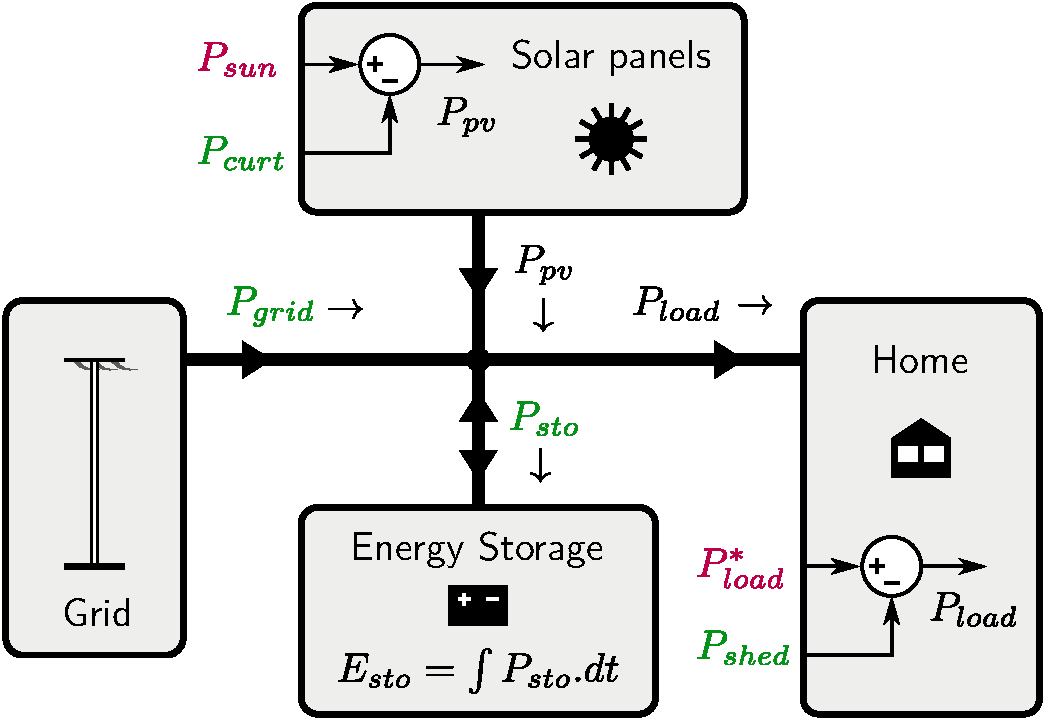
\includegraphics[width=0.9\columnwidth]{figures/solar_home.pdf}
        \end{center}

        \caption{Modèle en flux d'énergie de la maison solaire.
        Variables de décision en vert, données externes en rouge (potentiel solaire et consommation souhaitée), variables internes en noir.
        La consommation du foyer $P_{load}^*$, imposée, est couverte par 3 sources:
        le réseau électrique, des panneaux solaires (délestables)
        et un système de stockage.
        En dernier recours, la consommation de la maison peut être délestée.
        }
        \label{fig:solhome}
\end{figure}

Pour illustrer les différentes méthodes de gestion d'énergie à comparer,
nous avons choisi un système ``banc de test'' qui soit à la fois simple et concret.
Nous considérons une maison solaire modélisée par
des flux d'énergie (figure \ref{fig:solhome}).
Il s'agit d'un modèle simple de système photovoltaïque avec stockage
pour l'autoconsommation d'un consommateur résidentiel connecté au réseau.
Le modèle s'exprime à temps discret (instant $k$ entier),
avec un pas de temps $\Delta_t$. On note $n$ la durée du test
en nombres de pas.

L'objectif de pilotage est la minimisation de la facture d'électricité,
c'est à dire le coût de l'énergie consommée du réseau:

\begin{equation} \label{eq:C_grid}
  C_{grid} = \sum_{k=1}^{n} c_{grid}(k)P_{grid}(k)
\end{equation}

où $c_{grid}$ est le prix de l'énergie (\texteuro/kWh), potentiellement variable,
mais connu à l'avance.
En plus du signal prix, connu, les données du problèmes (en rouge sur la figure) sont:

\begin{itemize}
 \item $P_{sun}$ : productible solaire, c'est-à-dire la production des panneaux en régime
MPPT\footnote{Maximum power point tracking}
 \item $P_{load}^*$ : consommation souhaitée par la maison
\end{itemize}

En revanche, ces deux signaux ne sont pas connus à l'avance :
ce sont des \emph{entrées incertaines}.
On note que le productible solaire est proportionnel
à la puissance nominale (puissance crête) des panneaux $P_{PVp}$ (kWc),
qui est un paramètre de dimensionnement et non d'optimisation.
Du point de vue de la gestion d'énergie, $P_{PVp}$ est donc fixée.

Les degrés de libertés du problème (en vert sur la figure) sont au nombre de quatre.
La puissance soutirée du réseau, $P_{grid}$,
est libre mais limitée à la puissance souscrite $P_{grid}^{max}$
et l'injection est interdite\footnote{
équivalent, du point de vue de l'optimisation, à autoriser l'injection, mais sans la rémunérer}:
%
\begin{equation}
  0 \leq P_{grid} \leq P_{grid}^{max}
\end{equation}
%
Le système de gestion d'énergie peut tirer profit de l'énergie, marginalement
gratuite, produite par les panneaux solaires $P_{pv}$.
Cette puissance est librement réglable entre 0 et $P_{sun}$ grâce à la variable
d'écrêtage $P_{curt}$ :
%
\begin{equation}
  P_{pv} = P_{sun} - P_{curt}, \text{ avec } 0 \leq P_{curt} \leq P_{sun}
\end{equation}

Le système de gestion peut enfin exploiter le degré de liberté offert par
le système de stockage qui permet de décaler, au moins partiellement,
la production solaire et la consommation.
Le stockage, dont on néglige les pertes, est modélisé par l'énergie qu'il contient:
%
\begin{equation}
  E_{sto}(k+1) = E_{sto}(k) + P_{sto}(k)\Delta_t
\end{equation}
%
et ce stockage a une capacité limitée $E_{rated}$ :
%
\begin{equation}
  0 \leq E_{sto} \leq E_{rated}
\end{equation}

Tous les flux sont liés par la conservation de l'énergie:

\begin{equation}
  P_{grid} + \underbrace{P_{sun} - P_{curt}}_{P_{pv}} = P_{load} + P_{sto}
\end{equation}

La consommation $P_{load}$ a vocation à suivre la consommation souhaitée $P_{load}^*$
(pas de charges ``intelligentes'' déplaçables), et dans tout cet article, ces deux
variables seront égales et donc assimilés.
Nous définissons cependant $P_{shed}$ comme un délestage de dernier
recours pour les situations critiques\footnote{faible puissance souscrite, lorsque
la batterie est vide et qu'il n'y a que peu de soleil} et qui permet
de ramener $P_{load}$ à zéro si nécessaire:
%
\begin{equation}
  P_{load} = P_{load}^* - P_{shed}, \text{ avec } 0 \leq P_{shed} \leq P_{load}^*
\end{equation}

Si ce quatrième degré de liberté doit être utilisé,
alors il faut l'ajouter comme pénalité dans la fonction coût \eqref{eq:C_grid}.

\subsection{Dimensionnement}

TO BE CONTINUED

Notons pour finir que la performance d'un tel système dépend totalement de son dimensionnement
(capacité de stockage, puissance des panneaux et  puissance souscrite).
La question du dimensionnement, bien qu'intéressante, n'étant pas l'objet de cet article,
le dimensionnement est fixé empiriquement.

Dimensionnement: $E_{rated}=13.5\,$kWh (Tesla Powerwall), $P_{pv}^{max}=3\,$kW\textsubscript{c} (permet, en cumul annuel, de couvrir 64\% de la consommation du foyer présenté ci-après).

\subsection{Banc de test open source}

La description de ce modèle ainsi que les données temporelles nécessaires sont
disponibles en open source dans un dépôt GitHub \href{https://github.com/pierre-haessig/solarhome-control-bench}{solarhome-control-bench}.
Ce dépôt contient également les méthodes de gestion d'énergie présentées dans cet article.

Il a vocation à contenir des exemples dans les langages de programmation les plus utilisés pour ce type de problème:
Matlab, Python et Julia...

\subsection{Données de la maison solaire}

Nous utilisons le jeu de \emph{données réelles et ouvert} ``\href{https://www.ausgrid.com.au/Common/About-us/Corporate-information/Data-to-share/Solar-home-electricity-data.aspx}{Solar home electricity data}'' de l'opérateur Ausgrid (réseau de Sydney et sa région, Australie).
Il contient 3 années de consommation et production, au pas demi-horaire, de 300 clients résidentiels disposants de panneaux PV.

Pour notre banc de test, nous avons sélectionné un client sans charge pilotable\footnote{
  la description détaillée de ce choix est fournie dans le fichier \href{https://github.com/pierre-haessig/solarhome-control-bench/blob/master/data/README.md}{data/README.md} du dépôt, avec plusieurs graphiques supplémentaires.}.
Nous avons choisi 7 jours consécutifs de test représentés figure \ref{fig:testdata} (après mise à l'échelle à 3 kW\textsubscript{c} de son installation PV).

Les données des 30 jours précédents sont également disponibles pour une phase d'apprentissage,
par exemple pour régler la prévision d'une commande prédictive.


\begin{figure}[!ht]
        \begin{center}
                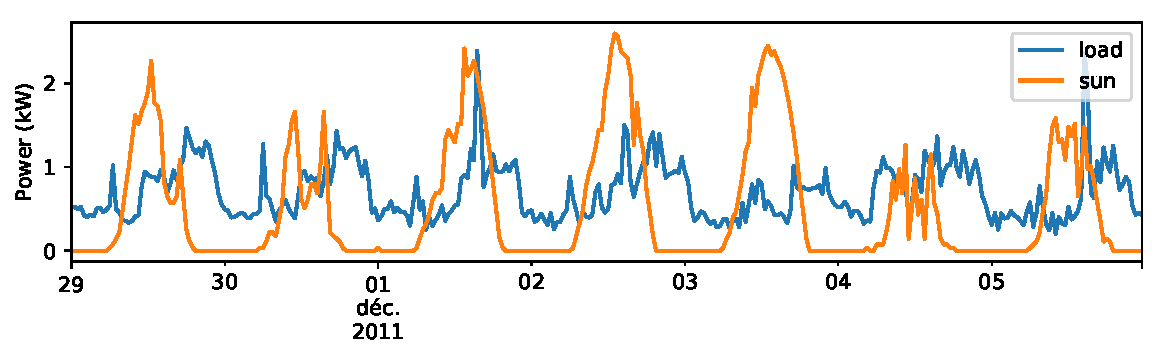
\includegraphics[width=1\columnwidth]{figures/data_week_2011-11-29.pdf}
        \end{center}

        \caption{Consommation et production PV durant les 7 jours de test
        }
        \label{fig:testdata}
\end{figure}


\section{Approches d'optimisation}
\label{s:opt_meth}

L'article final décrira les différentes méthodes comparées pour la gestion de la maison solaire,
avec les résultats obtenus.

\subsection{Programmation dynamique}
Bon cadre théorique pour poser un problème de gestion avec entrées incertaines (stochastique).
Point particulier: nécessite une modélisation des incertitudes par un \emph{processus markovien}\cite{Haessig:2013:ESPy}.
L'implémentation numérique est impossible si la dimension de l'état est trop grande (>4).


\subsection{Optimisation déterministe anticipative}

Un piège courant consiste à optimiser la gestion avec une connaissance parfaite des entrées.
Le résultat (figure \ref{fig:anticip}) est une surévaluation de la performance (e.g. aucun délestage de la production solaire).

%\cite{Rigo-Mariani:2014:SGE}
% poster µgrid powertech 2015 ?

\begin{figure}[!ht]
        \begin{center}
                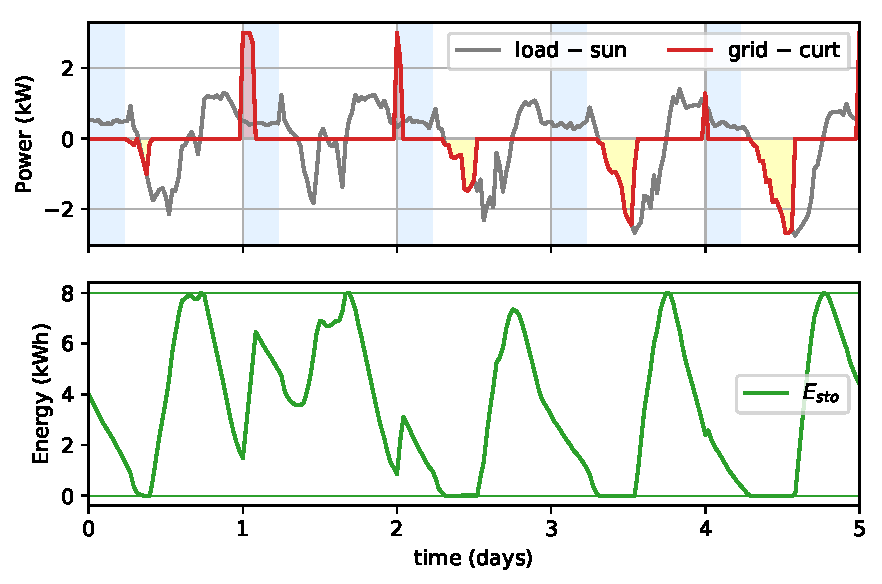
\includegraphics[width=1\columnwidth]{figures/julia_anticipative.pdf}
        \end{center}

        \caption{Gestion d'énergie par optimisation déterministe anticipative. La performance est surestimée
        (aucun délestage de production solaire).
        }
        \label{fig:anticip}
\end{figure}

\subsection{Commande prédictive (MPC)}
La commande prédictive (MPC) utilise une \emph{prévision ponctuelle (moyenne)} des entrées incertaines.
Elle compense l'erreur de prévision en répétant l'optimisation sur un \emph{horizon glissant}.
L'implémentation numérique est efficace si le problème d'optimisation est linéaire (ou en tout cas convexe),
ce qui est le cas ici.

Des variantes du MPC déterministe existent pour mieux faire face à l'incertain: le MPC stochastique,
qui utilise un \emph{ensemble de scénarios}, éventuellement avec un ``recours affine''.

%\subsection{MPC stochastique et robuste}

%une amélioration du MPC déterministe.

% \subsection{Commande prédictive non-linéaire}
% 
% Optimica JModelica.org \cite{Akesson:2010:CCE}
% 
% sareni sge 2014 \cite{Rigo-Mariani:2014:SGE} : optim linéaire puis reprojection.


\section{Conclusions}

Le banc de test pour la gestion d'énergie d'une maison solaire
doit permettre de faciliter l'accès à une palette de méthode de gestion
sur un exemple simple mais réaliste (e.g. données de production solaire et de consommation réelles).

Perspectives : ce banc de test pour la gestion d'énergie,
à dimensionnement fixé, est une première étape pour l'étude des méthodes
de dimensionnement optimal qui prennent en compte l'optimisation de la loi de gestion
\cite{Haessig:2014:SGE}.

% structure de décision dans un contexte multi-agent (pas abordé ici
% car focus sur optimisation d'un système individuel) : centralisé, distribué,
% mécanisme de prix, multi-agent...

\bibliographystyle{IEEEtran}
\bibliography{00_References}

\end{document}